\subsection{Implementierung des GUI}\label{l:implementierung-gui}

Im Prototypen wurden das GUI als reine JavaScript-Anwendung umgesetzt. Als Framework für den Aufbau der Anwendung wurde \trademark{Backbone.js}\footnote{\url{http://backbonejs.org/}} eingesetzt. 

\subsubsection{Komponenten}

\trademark{Backbone.js} stellt Basisklassen für Models, Views und Collections (Listen von Models) zur Verfügung, die mit Hilfe eines zentralen Routers zu einer Anwendung verbunden werden können, die mit einer RESTful-API kommunziert. Der Router übernimmt dabei die Aufgabe, abhängig von der URL im Browser zu steuern, welche View gerade eingezeigt wird. 

Um die einzelnen Bestandteile der Anwendung möglichst modular zu halten und Ladezeiten so kurz wie möglich zu halten, kommt \trademark{require.js}\footnote{\url{http://requirejs.org/}} zum Einsatz, mit dessen Hilfe es möglich ist, nur die für den aktuellen Code-Pfad nötigen Abhängigkeiten zu laden. Neben dem Nachladen von Ja\-va\-Scr\-ipt-Code ist es damit auch möglich HTML-Dateien nachzuladen, dies wird in der Implementierung dazu verwendet, den HTML-Code zur Darstellung der Anwendung ebenfalls modular und nur bei Bedarf nachzuladen. Dies ermöglich zudem eine saubere Trennung zwischen der Darstellungslogik, die in JavaScript implementiert ist und dem zugehörigen HTML-Quellcode. \trademark{Underscore.js}\footnote{\url{http://underscore.org/}}, auf dem \trademark{Backbone.js} aufbaut, liefert hierzu einfache Templating-Funktionen.

Zur Realisierung der GUI-Funktionalität wurde \trademark{Twitter Bootstrap}\footnote{\url{http://twitter.github.com/bootstrap/}} eingesetzt, ein HTML5-Framework, das für viele GUI-Elemente bereits vorgefertigte Darstellungen bietet. Einige Elemente werden mit Hilfe von JavaScript mit erweiterter Funktionalität versehen, in \trademark{Twitter Bootstrap} kommt dabei \trademark{JQuery}\footnote{\url{http://jquery.com/}} zum Einsatz. \trademark{Twitter Bootstrap} ermöglich von sich aus das GUI \emph{responsive} zu implementieren, d.h. dass keine festen Maßangaben verwendet werden. So ist eine saubere Darstellung auf vielen unterschiedlichen Endgeräte sichergestellt. Mit Hilfe von \emph{CSS media queries} können einfach Anpassung für bestimmte Bildschirmgrößen implementiert werden.

Alle genannten Komponenten sind umfangreich getestet und funktionieren in allen aktuellen Browsern und sind auch abwärtskompatibel zu älteren Browsern.

\setlength\fboxsep{2pt}
\setlength\fboxrule{0.5pt}

\begin{center}
\fbox{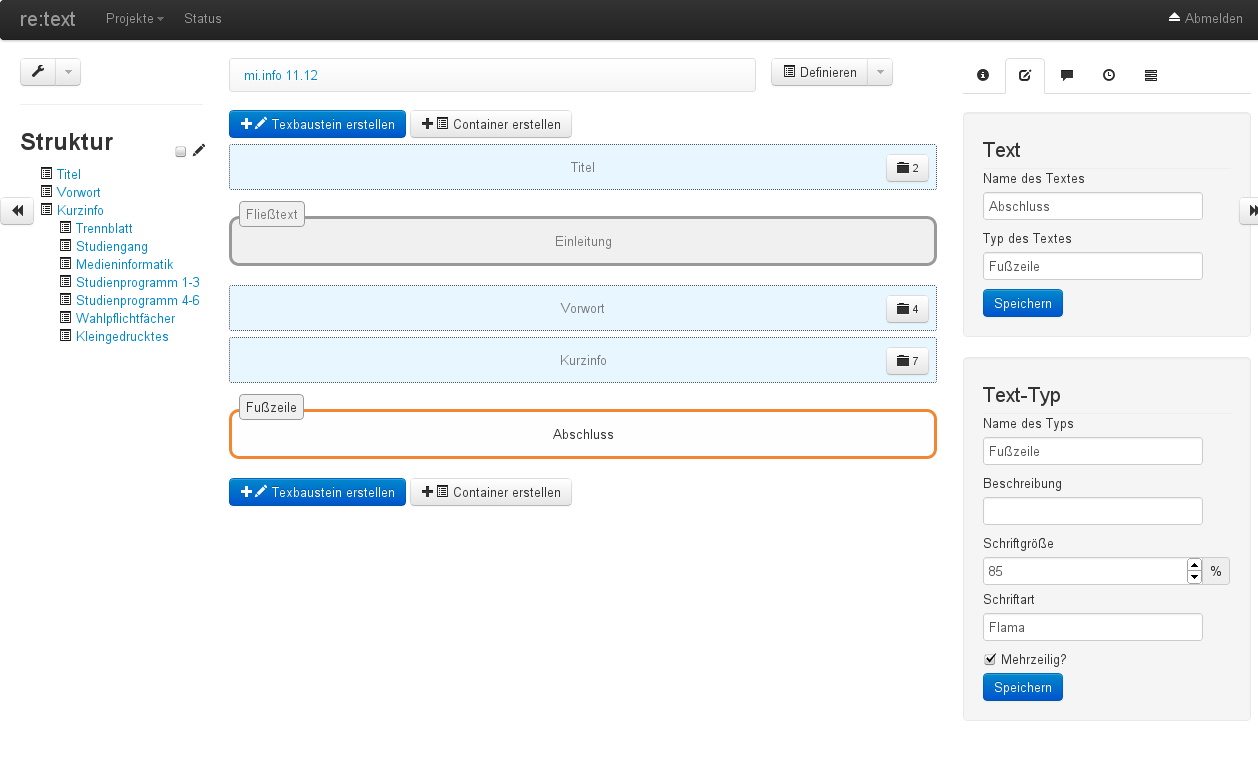
\includegraphics[width=\textwidth]{media/screenshots/app.png}}
\captionof{figure}{GUI des Prototypen}\label{chart:gui-prototyp}
\end{center}

Abbildung \ref{chart:gui-prototyp} zeigt den Aufbau des GUI des Prototypen beispielhaft in der Ansicht zur Definition des Produktes (vgl. Abschnitt \ref{l:gui-definition} / \pageref{l:gui-definition}). Die Anordnung der Elemente aus dem Entwurf wurde weitgehend beibehalten. Unterschiede resultieren aus im Prototyp nicht implementierte Funktionen, die nicht mit Platzhalter-Elementen dargestellt werden, sondern entfallen. Weitere Screenshots finden sich in Anhang~\ref{l:screenshots} · S.\pageref{l:screenshots}.

\subsubsection{Klassendiagramm}

\begin{center}
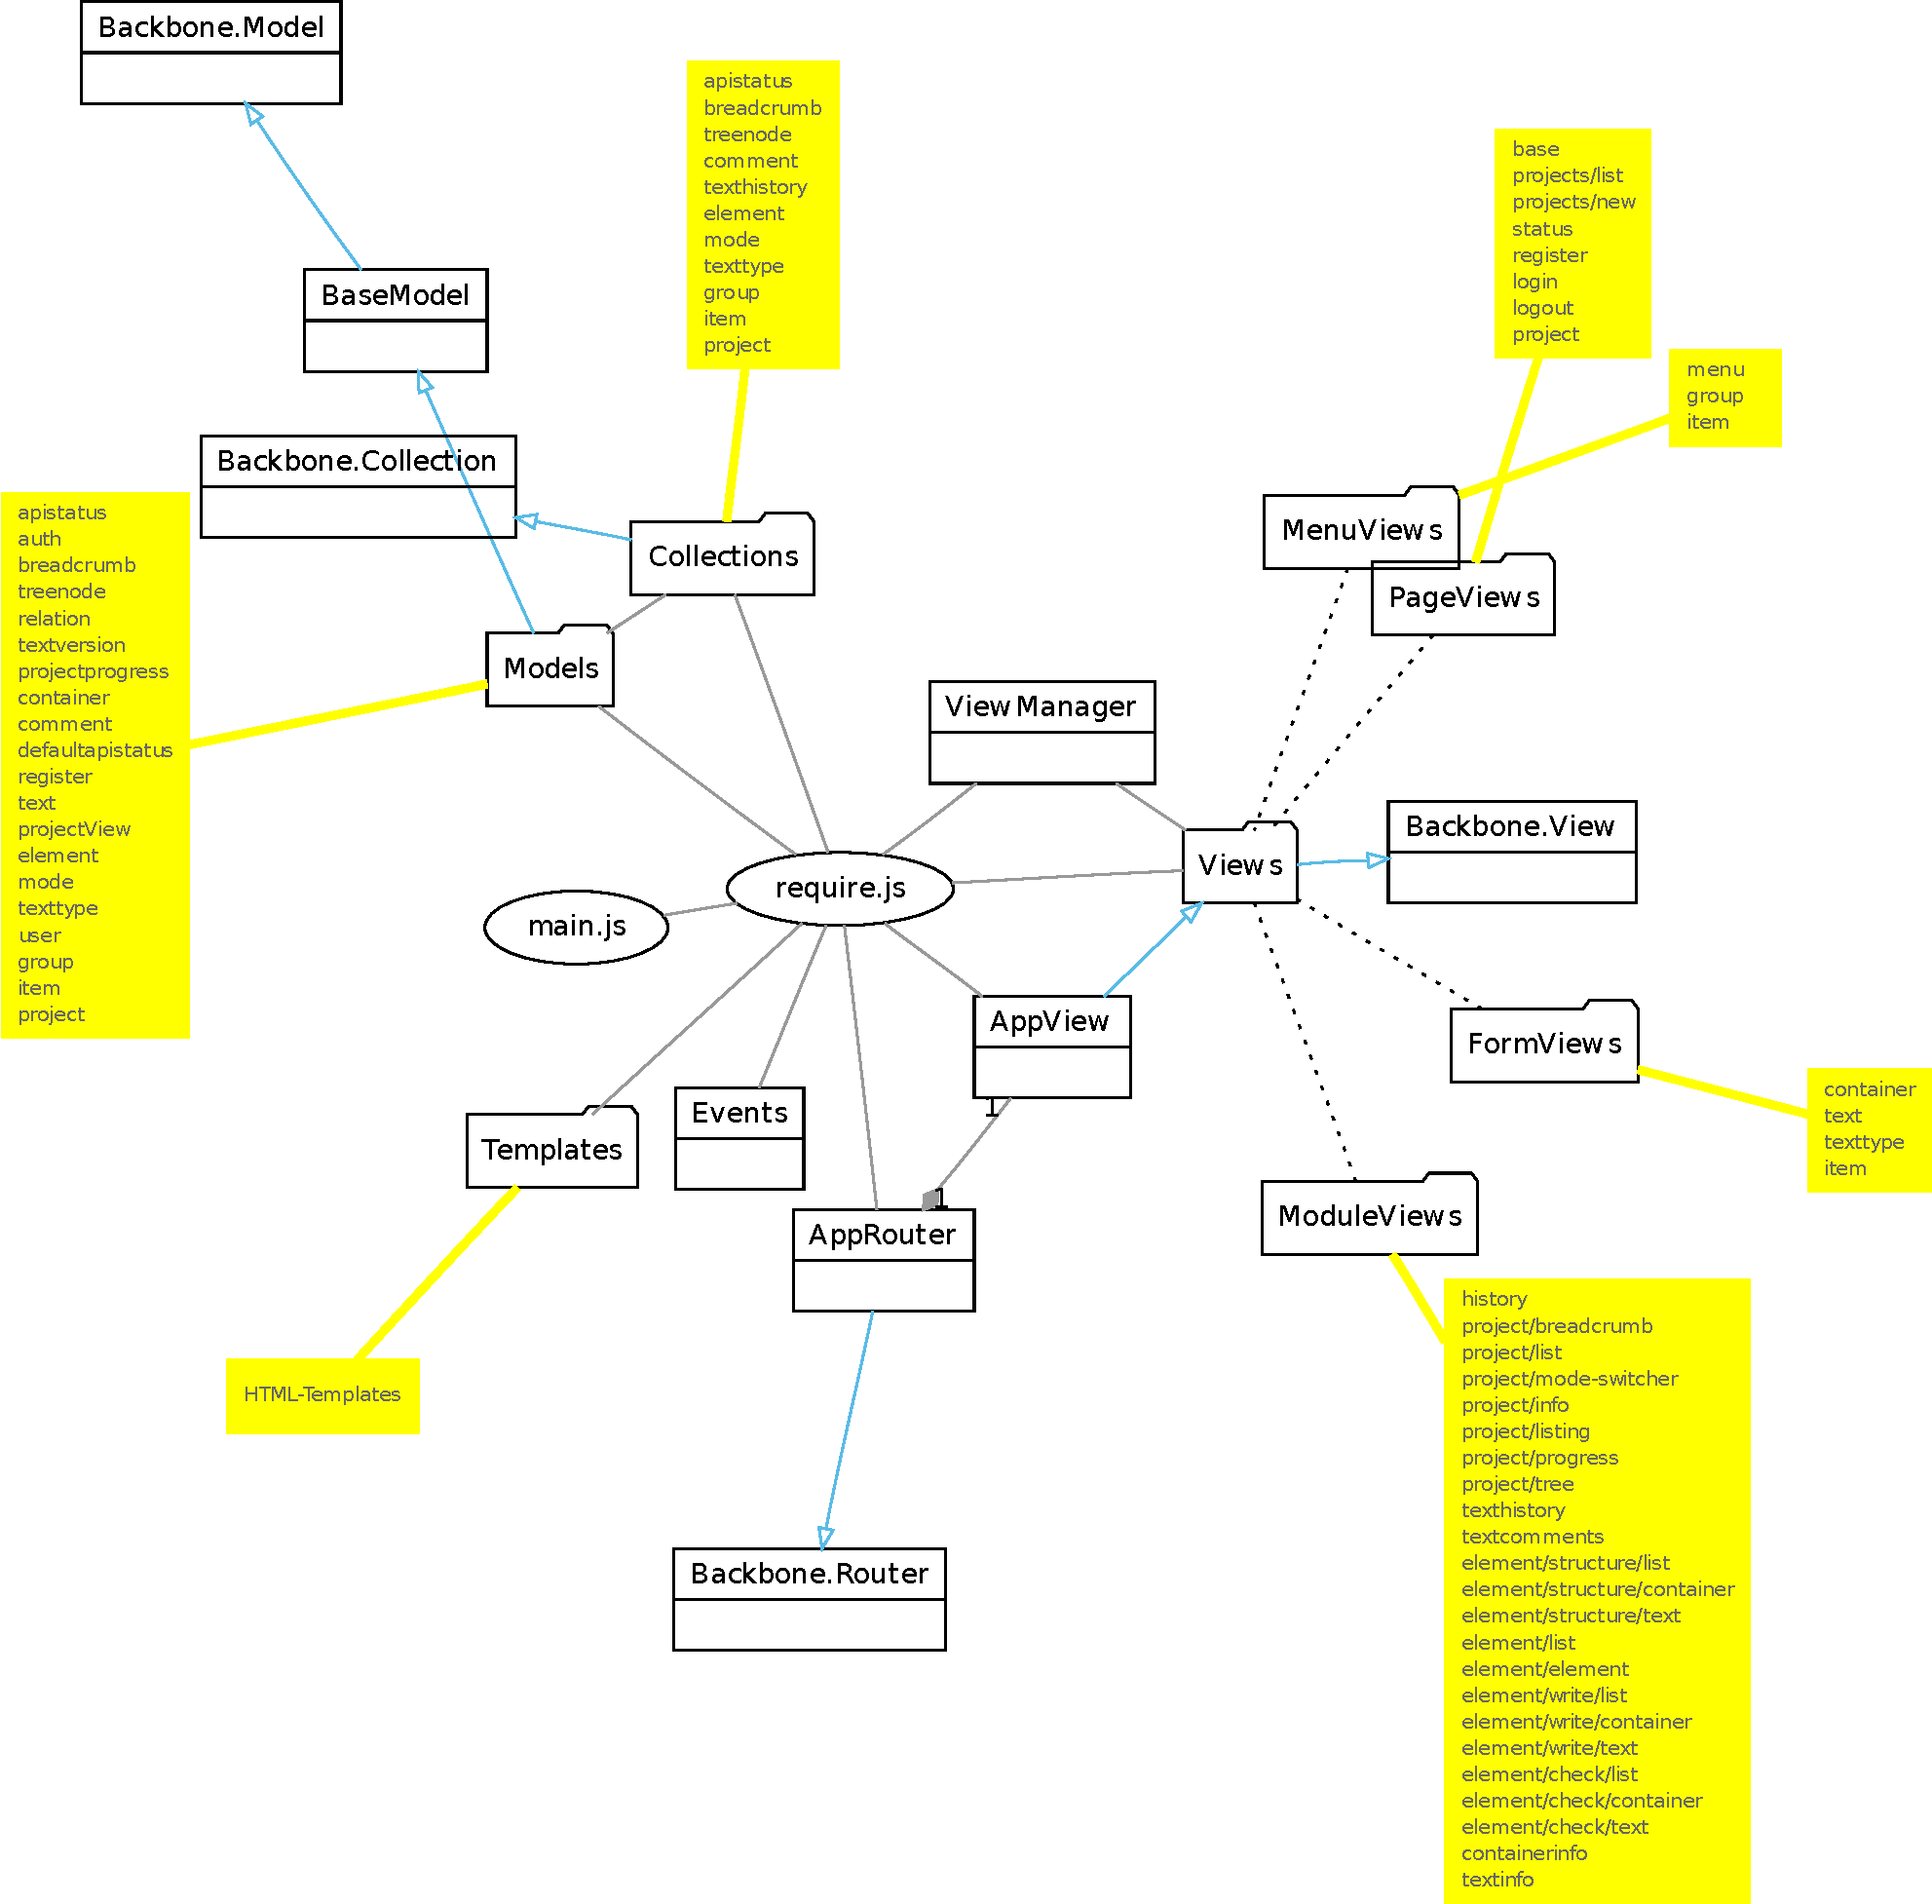
\includegraphics[width=\textwidth]{media/prototyp-gui-klassendiagramm.pdf}
\captionof{figure}{GUI-Klassendiagramm des Prototypen}\label{chart:prototyp-gui-klassendiagramm}
\end{center}

Abbildung \ref{chart:prototyp-gui-klassendiagramm} zeigt das Klassendiagramm der browserbasierten Anwendung. Zentraler Einstiegspunkt ist die JavaScript-Datein \texttt{main.js}, die die Anwendung initialisiert. Dazu lädt sie mit Hilfe von \texttt{require.js} die notwendigen Komponenten. Dabei handelt es sich zum einem um die \texttt{AppView}, die grundlegende Zustände der Anwendung verwaltet und den \texttt{AppRouter}, der je nach aktueller Route die jeweilige \texttt{PageView} initialisiert und anzeigt. Die \texttt{PageViews} erzeigen danach wiederum eiogenständig die von ihnen benötigten Ansichten (\texttt{ModuleViews}, \texttt{MenuViews} und \texttt{FormViews}) und Laden die dafür benötigten Daten mithilfe der \texttt{Models} und \texttt{Collections} -- in \trademark{Backbone.js} sind \emph{Views} eigentlich Controller, eine Trennung zwischen Darstellungslogik und Businesslogik ist nicht vorgesehen. Den HTML-Quellcode zur Darstellung laden die Views ebenfalls selbständig aus dem \texttt{Templates} nach. Abhängigkeiten wie JavaScript-Objekte und Templates werden dabei zentral von \trademark{require.js} bereitgestellt, dass damit die Aufgabe eines DI-Containers übernimmt und praktisch auch so verwendet werden kann.

Die Kommunikation mit der API wird durch die \trademark{Backbone.js}-Klassen \texttt{Backbone.Model} und \texttt{Backbone.Collection} abstrahiert, die RESTful-APIs ansprechen können, die dem CRUD-Paradigma entsprechen. Siehe dazu die Beschreibung der API-Implementierung in Abschnitt \ref{l:api-implementierung} · S.\pageref{l:api-implementierung}.
